\chapter{Theory}

\section{Bias point and class operation}
The bias point, or working point, of an amplifier determines which class the amplifier is, which in turn tells us something about the amplifiers efficiency, linearity and quiescent current. There is a wide variety of classes, the most common being class A, AB, B and C. 
Class A amplifiers have the highest quiescent current, the best linearity and the lowest efficiency (maximum theoretical efficiency of 50\% ). 
Class B amplifiers have no quiescent current, maximum theoretical efficiency of 78\% , but only conducts the positive half-period of a signal. 
Class AB is a hybrid between class A and B, sacrificing some of the efficiency of the class B amplifier, but gaining some of the linearity of the class A. 
Class C amplifiers are the most efficient of the four, having a maximum theoretical efficiency of almost 90\% . But they conduct for less than 50\%  of the signal cycle, typically they only conduct for a third of the cycle or less.
If the input signal of the amplifier is sufficiently small, one can bias the amplifier as an AB class, thus reducing quiescent current while still have class A operation in terms of linearity.

Once a class has been chosen, the bias point can be determined by examining the I-V characteristics of the transistor. By drawing a loadline going from the drain-source voltage on the X axis, to the drain saturation current on the Y axis, we get a linear line crossing the different gate-source voltage curves. See figure~\ref{fig:fig_Load_line}. By choosing a bias point along this linear curve, we can predict both quiescent current and voltage. The bias point for a class A amplifier will approximately be at Vds/2. The closer you move the bias point towards the maximum Vds voltage, the lower the class you get. This is because the loadline represents the current through and voltage across the transistors equivalent resistor.

\begin{figure}[H]
	  \centering
	  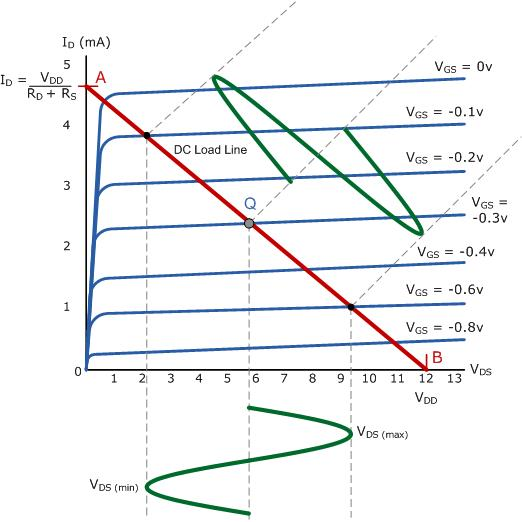
\includegraphics[width=0.75\textwidth]{img/Load_line_graphics}
	  \caption{Load line for class A amplifier}
	  \label{fig:fig_Load_line}
\end{figure}

\section{Efficiency}
There are several ways of expressing amplifier efficiency, the most common in the RF community being power added efficiency (PAE). PAE takes into account both the DC to RF power conversion, as well as the RF power delivered into the input of the device.

\begin{equation}
	PAE=\frac{P_{RFout}-P_{RFin}}{P_{DC}}=\frac{P_{RFout}-P_{RFin}}{V_{DC} \times I_{DC}} 
\end{equation}
By subtracting the power added to the input of the device from the output power, we get a better indication of the actual DC to RF power conversion. For low gain amplifiers the input power can be substantial and using drain efficiency (which does not take input power into consideration), will in these cases give a falsely high efficiency.
\section{Linearity}
Linearity is an important factor to consider when designing an amplifier. A linear amplifier will amplify a small input signal and a large input signal by the same amount, but better linearity often comes at the cost of efficiency, as the quiescent current must be increased. To better see the linearity of a transistor one can plot the drain current as a function of the gate-source voltage. This will produce a characteristic plot which shows how linear the transistor is for certain regions of the input signal.
\begin{figure}[H]
	  \centering
	  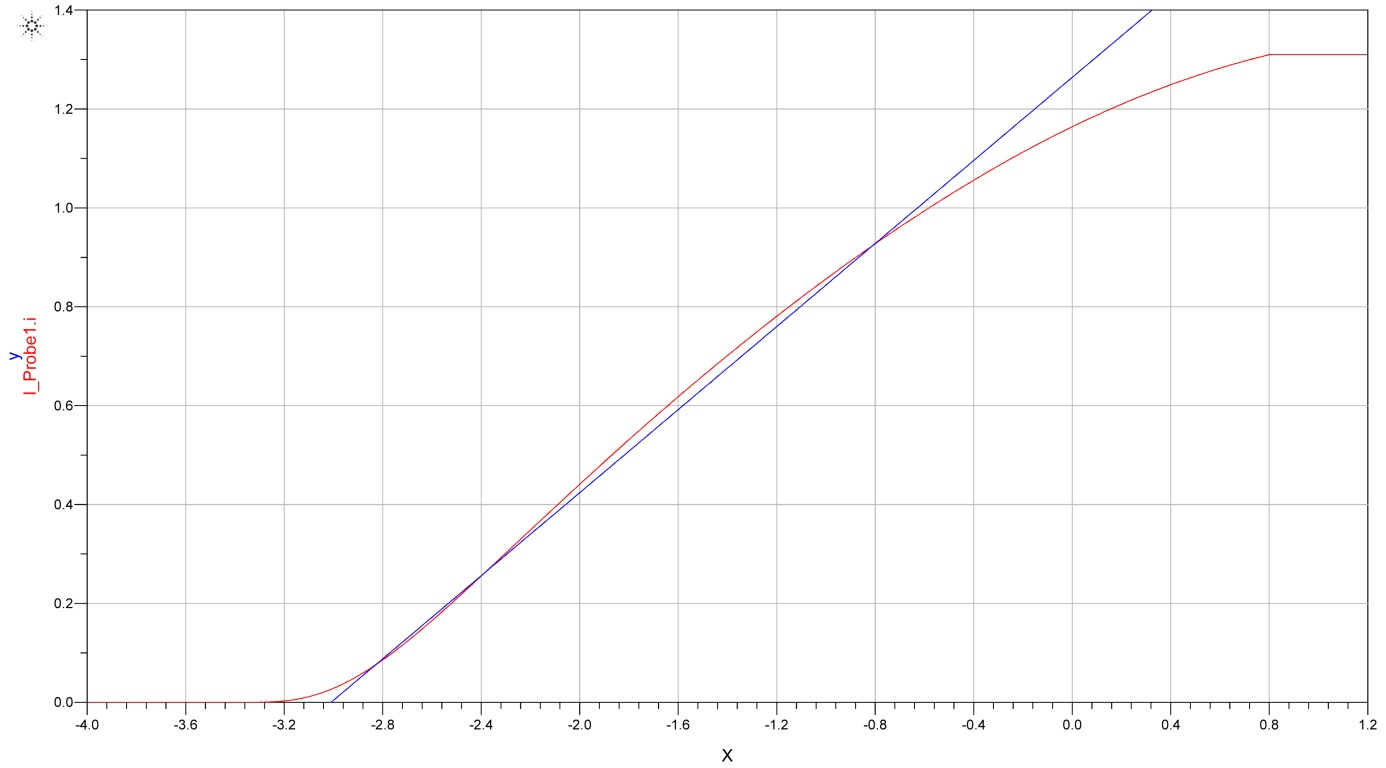
\includegraphics[width=0.75\textwidth]{img/Linearity_curve}
	  \caption{Drain current plotted vs gate-source voltage (shown in red). The blue line is a linear curve, making it easier to see the linearity of the device}
	  \label{fig:fig_Linearity_line}
\end{figure}
We can see in figure~\ref{fig:fig_Linearity_line} the most linear area for this device approximately lie between $-2.8V$ and $-2.4V$. Biasing the transistor for $-2.6V$ would offer the most linear response as long as the amplitude of the input signal does not exceed $0.2V$ in the negative half period, which would drive the gate-source voltage below $-2.8$ volts and into cut-off. 
\section{S-parameters}
S-parameters, or scattering parameters, are a set of 4 parameters which describe a systems electrical behavior. When referring to two-port amplifiers we use the parameters $S_{11},\, S_{12},\, S_{21}$ and $S_{22}$.
\begin{figure}[H]
	  \centering
	  
\includegraphics[width=0.75\textwidth]{img/S_parameter_image}
	  \caption{two-port signals for s-parameters}
	  \label{fig:fig_sparam_vis}
\end{figure}
 $S_{11}$ refers to the reflection of a input signal in $a_1$, returning back to the source through $b_1$, $S_{12}$ refers to the reverse voltage gain, $S_{21}$ refers to the forward voltage gain and $S_{22}$ refers to the reflection of the output signal in b2 back through $a_2$.
 The relationship between incident power, reflected power and the S-parameter matrix is given by the equation:
 \begin{equation}
	\begin{bmatrix}
	b_1\\
	b_2
	\end{bmatrix}
	=
	\begin{bmatrix}
	S_{11} & S_{12}\\
	S_{21} & S_{22}
	\end{bmatrix}
	\times
	\begin{bmatrix}
	a_1\\
	a_2
	\end{bmatrix}
 \end{equation}

\section{Stability}
Amplifier stability refers to the amplifiers tendency to oscillate, which is something we strive to prevent. Oscillations occure when the "reflected" value of an incident voltage (at either input or output) is larger than 1.
\begin{figure}[H]
	  \centering
	  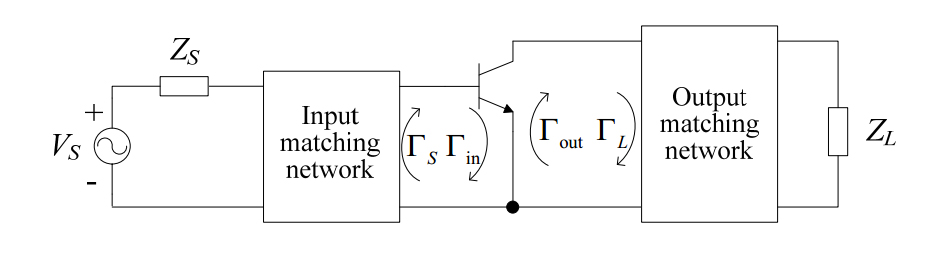
\includegraphics[width=0.75\textwidth]{img/Reflection_example}
	  \caption{reflections of an amplifiers circuit}
	  \label{fig:fig_reflection_ex}
\end{figure}
In Figure~\ref{fig:fig_reflection_ex} the $\Gamma_s$ refers to the reflection of the returning signal to the source, $\Gamma_{in}$ is the reflection of the input, $\Gamma_{out}$ is the reflection of returning signals at the output and $\Gamma_L$ is the reflection of signals to the load. If the input and output matching networks are passive, then $|\Gamma_s|<1$ and $|\Gamma_L|<1$. The circuit can be unstable if $|\Gamma_{in}|>1$ and $|\Gamma_{out}|>1$. 

By expressing $|\Gamma_{in}|$ and $|\Gamma_{out}|$ as functions of $\Gamma_L$  and $\Gamma_s$ respectively, in combination with the S-parameters, we can find an expression for a circle in the smith chart which represents the border between the region of stability and instability at input and output. These are called stability circles, and can tell us at what impedances the device is stable, or unstable.
There are two main measures of stability, the K-factor and the mu-factors:
\begin{equation}
K=\frac{1-|S_{11}|^2-|S_{22}|^2+|\nabla |^2}{2\times |S_{21}\times S_{12}|},\, \nabla =S_{11}\times S_{22}-S_{12}\times S_{21}
\end{equation}
The K-factor tells us whether or not the amplifier is stable for a specific frequency, which means we need to evaluate the K-factor from 0Hz (DC) to the highest frequency the amplifier can oscillate at. If K>1 the amplifier is stable for the specific frequency. If K>1 for all frequencies we say the amplifier is unconditionally stable, if there are frequencies where K<1, we say the amplifier is conditionally stable.  The K-factor tells us if the amplifier is stable, but not by how much. A larger value of K does not indicate a more stable amplifier. When designing an amplifier it is useful to know how stable our device is, so we can take variations in the manufacturing process into consideration. For this purpose we use the mu-factors:
\begin{equation}
\mu=\frac{1-|S_{11}|^2}{|S_{22}-\nabla \times S_{11}^*|+|S_{12}\times S_{21}|}>1
\end{equation}
\begin{equation}
\mu_{prime}=\frac{1-|S_{22}|^2}{|S_{11}-\nabla \times S_{22}^*|+|S_{12}\times S_{21}|}>1
\end{equation}
The mu-factors tell us the distance from the center of the smith chart, to the edge of the stability circle. Mu shows this distance for the output, while mu-prime shows the same for the input. If the value of the factor is above 1 the device is unconditionally stable for the given frequency, and the larger the values of the factors are the more stable a device is. This way we can add some margin to our amplifiers stability, to ensure it is stable after the manufacturing process.
\section{Quarter wave transformation}
For high frequency applications great care must be taken when designing the transmission lines on the PCB layout, as the wavelength of the signals are comparable to the lengths of the PCB traces. This causes the transmission lines to have significant capacitive or inductive effects on the signal, depending on the trace length. This allows us to create RLC circuits without the use of lumped components by strategically choosing the length, width and shape of each trace. A transmission line with a length equal to the signal wavelength will result in a $360^\circ$ phase-shift in the signal. Similarly a trace with a length equal to a quarter of the wavelength would result in a $90^\circ$ phase shift. If we have an open stub with a length equal to $^1/_4$ wavelength, the impedance at the open end of the stub would be infinite. The voltage at that point would be high, while the current would be zero. At the other end of the stub, the phase of the signal would have shifted  $90^\circ$, and the stub would appear to be a short circuit. This effect is highly frequency dependent, and the circuit can thusly be designed to only affect the signals of our choosing.
\section{Matching}
To affect stability, performance and efficiency matching networks are created at the amplifier input and output to adjust the impedance “seen” by the source and load. See figure~\ref{fig_reflection_ex}. For maximum power transfer, the output and input matching networks are matched to the characteristic impedance at the source and load, usually $50\Omega$ and sometimes $75\Omega$. For maximum gain or low noise the networks must be intentionally designed with mismatches compared to the characteristic impedances. By tweaking the networks matching, we can find a balance between the desired properties.

\section{Small signal vs large signal}
Small and large signal analysis is used to evaluate the amplifier design once a bias point has been chosen. When performing small signal analysis we use the chosen bias point, and look at the amplifiers response in the linear area of operation. Here we can assess the amplifiers gain, linearity and efficiency for signals well within the amplifiers capabilities.
When looking at large signal analysis on the other hand we use large input signals to drive the amplifier into compression, and the non-linear area of operation. Here we can find the 1 dB compression point, the input signal level at which the amplifiers amplification is reduced by 1 dB.

\section{Intermodulation distortion}
Intermodulation distortion (IMD) is found when performing a two tone test on a non-linear device. A linear amplifier would produce two tones at the same frequencies as the input signals but amplified in power. A non-linear device will create harmonics, and if subjected to a two-tone test it will also create signals which are the result of intermodulation (see figure~\ref{fig_distortion_vis}). As can be seen in the figure the intermodulation distortion components are caused by the summation (both additive and subtractive) of the harmonics of the two tones, creating distortion around the fundamental frequencies, as well as between the second and third harmonics.
\begin{figure}[H]
	  \centering
	  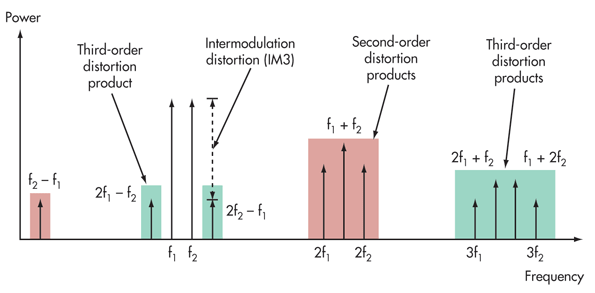
\includegraphics[width=0.75\textwidth]{img/Intermodulation_distortion}
	  \caption{Intermodulation distortion visualization}
	  \label{fig:fig_distortion_vis}
\end{figure}